% fig16-ged-bimodality.tex
% Structural drift across solved interventions in the paper-freeze cohort
\documentclass[tikz,border=18pt]{standalone}
% common-styles.tex
% Shared TikZ styles for wonton-proof paper figures

\usepackage{silence}
\WarningFilter{latex}{Missing character} 
\tracinglostchars=0 % Suppress engine-level "Missing character" warnings

\usepackage{fontspec}
\usepackage{unicode-math}

% Use filenames for reliability with Tectonic
\setmainfont{LibertinusSerif-Regular.otf}[
    BoldFont=LibertinusSerif-Bold.otf,
    ItalicFont=LibertinusSerif-Italic.otf,
    BoldItalicFont=LibertinusSerif-BoldItalic.otf
]
\setsansfont{LibertinusSans-Regular.otf}[
    BoldFont=LibertinusSans-Bold.otf,
    ItalicFont=LibertinusSans-Italic.otf
]
\setmonofont{LibertinusMono-Regular.otf}

% Try a more standard math font if LibertinusMath is causing nullfont issues
\setmathfont{LibertinusMath-Regular.otf}
% \setmathfont{latinmodern-math.otf}[range=digits] 

\usepackage{amsmath}
\usepackage{tikz}
\usepackage{forest}

\usetikzlibrary{
    arrows.meta,
    calc,
    decorations.pathreplacing,
    fit,
    positioning,
    shapes.geometric,
    shapes.misc,
    backgrounds,
    shadows.blur,
    fadings
}

% Color palette (muted, print-friendly)
\definecolor{ink}{RGB}{45,45,52}
\definecolor{muted}{RGB}{115,115,125}
\definecolor{highlight}{RGB}{198,120,44}
\definecolor{accentblue}{RGB}{86,130,178}
\definecolor{accentgreen}{RGB}{84,156,132}
\definecolor{blocked}{RGB}{140,75,75}
\definecolor{goalnode}{RGB}{255,255,255}
\definecolor{terminal}{RGB}{238,239,244}
\definecolor{deadnode}{RGB}{248,245,245}
\definecolor{flowbox}{RGB}{250,250,252}
\definecolor{basin1}{RGB}{224,234,248}
\definecolor{basin2}{RGB}{246,232,221}
\definecolor{basin3}{RGB}{228,242,234}
\definecolor{heatbase}{RGB}{86,130,178}

\tikzset{
    line cap=round,
    line join=round,
    pop/.style={
        blur shadow={shadow blur steps=5, shadow blur extra rounding=1.3pt}
    },
    base node/.style={
        rounded rectangle,
        draw=ink,
        line width=0.6pt,
        fill=goalnode,
        text=ink,
        minimum width=2.2cm,
        minimum height=0.7cm,
        align=center,
        pop
    },
    goal/.style={base node, fill=goalnode},
    terminal/.style={base node, fill=terminal, line width=0.9pt},
    dead/.style={base node, fill=deadnode, dashed},
    flowbox/.style={
        rectangle,
        draw=muted,
        rounded corners=3pt,
        fill=flowbox,
        minimum width=1.8cm,
        minimum height=0.6cm,
        align=center,
        font=\normalfont\small,
        text=ink,
        pop
    },
    decision/.style={
        diamond,
        draw=muted,
        fill=flowbox,
        aspect=2.4,
        font=\normalfont\small,
        inner sep=1pt,
        text=ink
    },
    protocolbox/.style={
        rectangle,
        draw=muted,
        rounded corners=4pt,
        fill=flowbox,
        minimum width=2cm,
        minimum height=0.8cm,
        font=\normalfont\small,
        align=center,
        text=ink
    },
    tactic/.style={
        ->,
        >=Stealth,
        draw=muted,
        line width=0.75pt
    },
    tacticlight/.style={
        ->,
        >=Stealth,
        draw=muted!45,
        dashed,
        line width=0.6pt
    },
    backprop/.style={
        ->,
        >=Stealth,
        draw=muted!70,
        dashed,
        line width=0.6pt
    },
    selected/.style={
        tactic,
        draw=highlight,
        line width=1.4pt
    },
    divergetactic/.style={
        tactic,
        draw=highlight,
        line width=1.4pt
    },
    divergenode/.style={
        base node,
        draw=highlight,
        line width=1.0pt
    },
    divergeblock/.style={
        blockedtactic,
        line width=1.2pt
    },
    blockedtactic/.style={
        tactic,
        draw=blocked,
        densely dashed
    },
    flowarrow/.style={
        ->,
        >=Stealth,
        draw=muted,
        line width=0.75pt
    },
    crosslink/.style={
        -,
        draw=muted!70,
        dotted,
        line width=0.6pt
    },
    annot/.style={
        font=\normalfont\footnotesize,
        text=muted
    },
    visit/.style={
        annot,
        font=\normalfont\scriptsize
    },
    annotbg/.style={
        annot,
        fill=white,
        inner sep=1.5pt
    },
    tacticlabel/.style={
        annot,
        font=\ttfamily\footnotesize,
        text=muted
    },
    formula/.style={
        font=\normalfont\footnotesize,
        draw=muted,
        rounded corners=2pt,
        fill=white,
        inner sep=3pt
    },
    paneltitle/.style={
        font=\normalfont\bfseries,
        text=ink
    },
    trajectory/.style={
        ->,
        draw=muted!70,
        line width=0.6pt
    }
}


\begin{document}
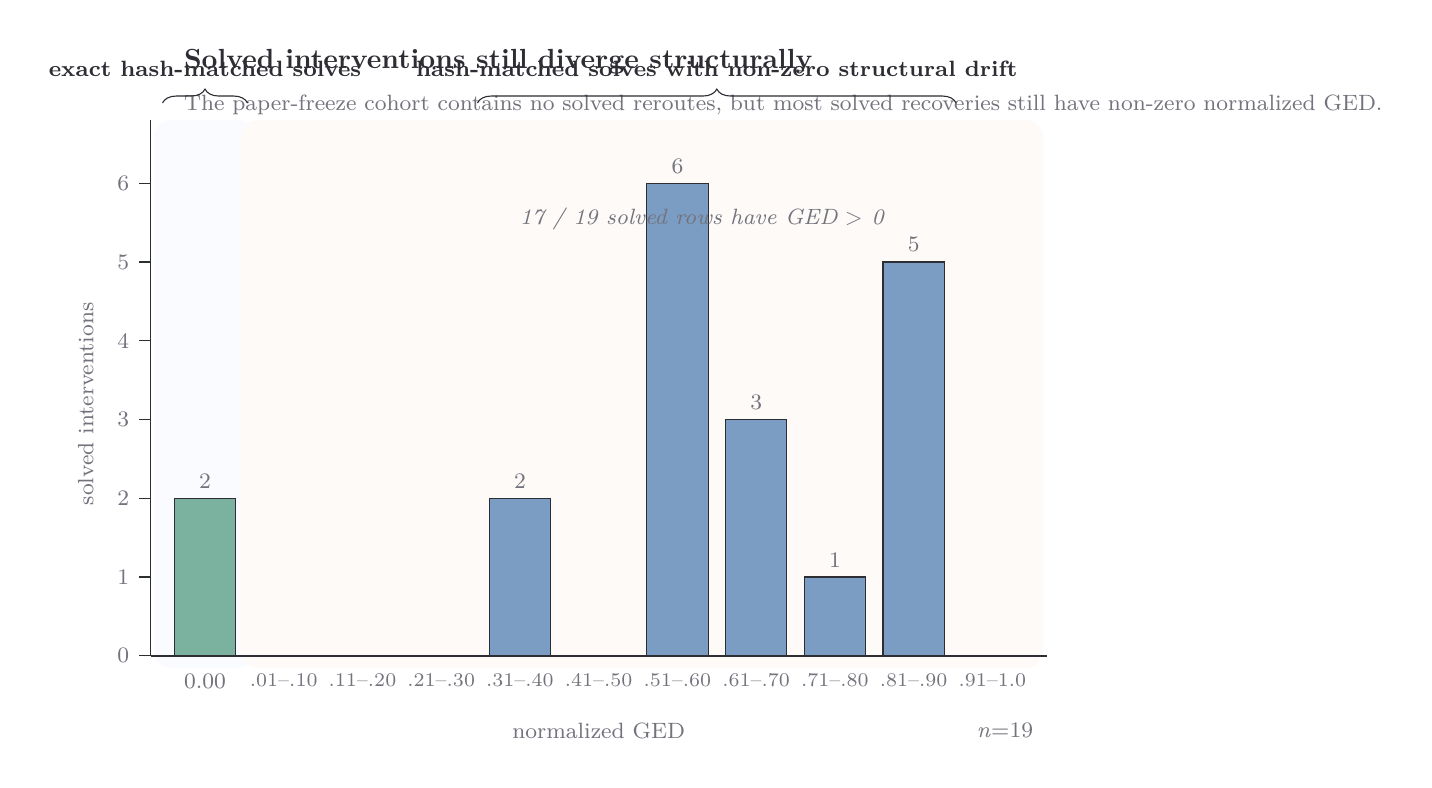
\begin{tikzpicture}[
    every node/.style={font=\small},
    show background rectangle,
    background rectangle/.style={fill=white}
]

\def\barwidth{0.78}
\def\barspacing{1.00}

% Counts from wonton_paper_closeout_v1 / paper_p2_interventions.jsonl
% Solved interventions (n = 19):
% 0.00=2, 0.31-0.40=2, 0.51-0.60=6, 0.61-0.70=3, 0.71-0.80=1, 0.81-0.90=5

\def\hA{2}
\def\hB{0}
\def\hC{0}
\def\hD{0}
\def\hE{2}
\def\hF{0}
\def\hG{6}
\def\hH{3}
\def\hI{1}
\def\hJ{5}
\def\hK{0}
\def\ymax{6.8}

\path[fill=basin1!18, rounded corners=6pt]
    (-0.25, -0.15) rectangle (0.25+\barwidth, \ymax);
\path[fill=basin2!20, rounded corners=6pt]
    (1*\barspacing-0.15, -0.15) rectangle (10*\barspacing+\barwidth+0.25, \ymax);

\node[paneltitle, anchor=west] at (0, 7.55) {Solved interventions still diverge structurally};
\node[annot, anchor=west] at (0, 7.0) {The paper-freeze cohort contains no solved reroutes, but most solved recoveries still have non-zero normalized GED.};

\fill[accentgreen!78] (0, 0) rectangle (\barwidth, \hA);
\fill[accentblue!78] (1*\barspacing, 0) rectangle (1*\barspacing+\barwidth, \hB);
\fill[accentblue!78] (2*\barspacing, 0) rectangle (2*\barspacing+\barwidth, \hC);
\fill[accentblue!78] (3*\barspacing, 0) rectangle (3*\barspacing+\barwidth, \hD);
\fill[accentblue!78] (4*\barspacing, 0) rectangle (4*\barspacing+\barwidth, \hE);
\fill[accentblue!78] (5*\barspacing, 0) rectangle (5*\barspacing+\barwidth, \hF);
\fill[accentblue!78] (6*\barspacing, 0) rectangle (6*\barspacing+\barwidth, \hG);
\fill[accentblue!78] (7*\barspacing, 0) rectangle (7*\barspacing+\barwidth, \hH);
\fill[accentblue!78] (8*\barspacing, 0) rectangle (8*\barspacing+\barwidth, \hI);
\fill[accentblue!78] (9*\barspacing, 0) rectangle (9*\barspacing+\barwidth, \hJ);
\fill[accentblue!78] (10*\barspacing, 0) rectangle (10*\barspacing+\barwidth, \hK);

\foreach \i/\h in {0/\hA,1/\hB,2/\hC,3/\hD,4/\hE,5/\hF,6/\hG,7/\hH,8/\hI,9/\hJ,10/\hK} {
    \draw[ink, line width=0.4pt] (\i*\barspacing, 0) rectangle (\i*\barspacing+\barwidth, \h);
}

\foreach \i/\h/\count in {
    0/\hA/2,
    4/\hE/2,
    6/\hG/6,
    7/\hH/3,
    8/\hI/1,
    9/\hJ/5
} {
    \node[annot, above] at (\i*\barspacing+\barwidth/2, \h) {\count};
}

\node[annot, below=3pt, align=center] at (0+\barwidth/2, 0) {0.00};
\node[annot, below=3pt, font=\normalfont\scriptsize, align=center] at (1*\barspacing+\barwidth/2, 0) {.01--.10};
\node[annot, below=3pt, font=\normalfont\scriptsize, align=center] at (2*\barspacing+\barwidth/2, 0) {.11--.20};
\node[annot, below=3pt, font=\normalfont\scriptsize, align=center] at (3*\barspacing+\barwidth/2, 0) {.21--.30};
\node[annot, below=3pt, font=\normalfont\scriptsize, align=center] at (4*\barspacing+\barwidth/2, 0) {.31--.40};
\node[annot, below=3pt, font=\normalfont\scriptsize, align=center] at (5*\barspacing+\barwidth/2, 0) {.41--.50};
\node[annot, below=3pt, font=\normalfont\scriptsize, align=center] at (6*\barspacing+\barwidth/2, 0) {.51--.60};
\node[annot, below=3pt, font=\normalfont\scriptsize, align=center] at (7*\barspacing+\barwidth/2, 0) {.61--.70};
\node[annot, below=3pt, font=\normalfont\scriptsize, align=center] at (8*\barspacing+\barwidth/2, 0) {.71--.80};
\node[annot, below=3pt, font=\normalfont\scriptsize, align=center] at (9*\barspacing+\barwidth/2, 0) {.81--.90};
\node[annot, below=3pt, font=\normalfont\scriptsize, align=center] at (10*\barspacing+\barwidth/2, 0) {.91--1.0};

\draw[ink, line width=0.6pt] (-0.3, 0) -- (10*\barspacing+\barwidth+0.3, 0);
\draw[ink, line width=0.6pt] (-0.3, 0) -- (-0.3, \ymax);
\node[annot, rotate=90, anchor=south] at (-0.9, 3.2) {solved interventions};

\foreach \y in {0,1,2,3,4,5,6} {
    \draw[ink, line width=0.4pt] (-0.3, \y) -- (-0.45, \y);
    \node[annot, left] at (-0.45, \y) {\y};
}

\node[annot] at (5*\barspacing+\barwidth/2, -0.95) {normalized GED};
\draw[decorate, decoration={brace, amplitude=5pt, raise=2pt}, ink]
    (-0.15, 6.95) -- (0.15+\barwidth, 6.95)
    node[midway, above=8pt, font=\normalfont\footnotesize\bfseries, text=ink] {exact hash-matched solves};
\draw[decorate, decoration={brace, amplitude=5pt, raise=2pt}, ink]
    (4*\barspacing-0.15, 6.95) -- (9*\barspacing+\barwidth+0.15, 6.95)
    node[midway, above=8pt, font=\normalfont\footnotesize\bfseries, text=ink] {hash-matched solves with non-zero structural drift};

\node[annot, text=muted, font=\normalfont\footnotesize\itshape] at (6.7, 5.55) {17 / 19 solved rows have GED $>$ 0};
\node[annot, anchor=east] at (10*\barspacing+\barwidth+0.25, -0.95) {\textit{n}=19};

\end{tikzpicture}
\end{document}
